\input ../SlidePreamble
\input ../preamble

\begin{document}

{\huge
  \centerline{\bf TTIC 31230,  Fundamentals of Deep Learning, Winter 2019}
  \vfill
  \centerline{David McAllester}
  \vfill
  \centerline{\bf The Fundamental Equations of Deep Learning}


\slide{Early History}

{\bf 1943}: McCullock and Pitts introduced the linear threshold ``neuron''.

\vfill
{\bf 1962}: Rosenblatt applies a ``Hebbian'' learning rule.  Novikoff proved the perceptron convergence theorem.

\vfill
{\bf 1969}: Minsky and Papert publish the book {\it Perceptrons}.

\vfill
The Perceptrons book greatly discourages work in artificial neural networks.  Symbolic methods dominate AI research through the 1970s.

\slide{80s Renaissance}

{\bf 1980}: Fukushima introduces the neocognitron (a form of CNN)

\vfill
{\bf 1984}: Valiant defines PAC learnability and stimulates learning theory. Wins Turing Award in 2010.

\vfill
{\bf 1985}: Hinton and Sejnowski introduce the Boltzman machine

\vfill
{\bf 1986}: Rummelhart, Hinton and Williams demonstrate empirical success with backpropagation (itself dating back to 1961).

\slide{90s and 00s: Research In the Shadows}

{\bf 1997}: Schmidhuber et al. introduce LSTMs

\vfill
{\bf 1998}: LeCunn introduces convolutional neural networks (CNNs) (LeNet).

\vfill
{\bf 2003}: Bengio introduces neural language modeling.

\slide{Current Era}

{\bf 2012}: Alexnet dominates the Imagenet computer vision challenge.

\vfill
Google speech recognition converts to deep learning.

\vfill
Both developments come out of Hinton's group in Toronto.

\vfill
{\bf 2013}: Refinement of AlexNet continues to dramatically improve computer vision.

\vfill
{\bf 2014}: Neural machine translation appears (Seq2Seq models).

\vfill
Variational auto-encoders (VAEs) appear.

\vfill
Graph networks for molecular property prediction appear.

\vfill
Dramatic improvement in computer vision and speech recognition continues.

\slide{Current Era}

{\bf 2015}: Google converts to neural machine translation leading to dramatic improvements.

\vfill
ResNet appears.  This makes yet another dramatic improvement in computer vision.

\vfill
Generative Adversarial Networks (GANs) appear.

\vfill
{\bf 2016}: Alphago defeats Lee Sedol.

\slide{Current Era}

{\bf 2017}: AlphaZero learns both go and chess at super-human levels in a mater of hours entirely form self-play and advances computer go far beyond human abilities.

\vfill
Unsupervised machine translation is demonstrated.

\vfill
Progressive GANs.

\vfill
{\bf 2018}: Unsupervised pre-training significantly improves a broad range of NLP tasks including question answering (but dialogue remains unsolved).

\vfill
AlphaFold revolutionizes protein structure prediction.

\slidetwo{What is a Deep Network?}
{VGG, Zisserman, 2014}

\centerline{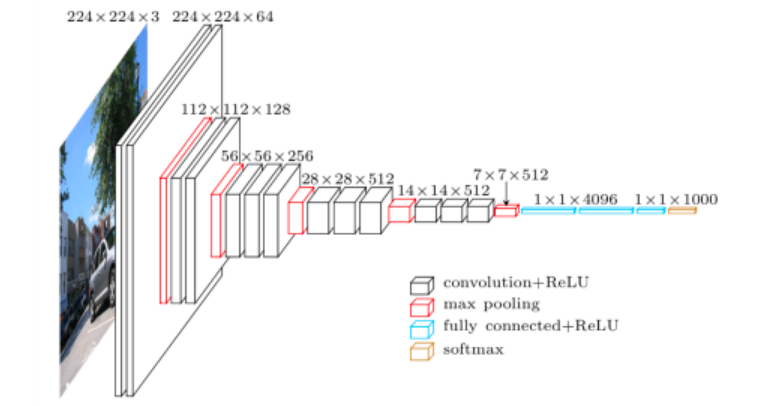
\includegraphics[width = 8.0in]{../images/VGG}}
\centerline{\large Davi Frossard}

\slide{What is a Deep Network?}

We assume some set ${\cal X}$ of possible inputs, some set ${\cal Y}$ of possible outputs,
and a parameter vector $\Phi \in \reals^d$.

\vfill
For a parameter vector $\Phi$, a given input $x \in {\cal X}$, and for each possible output $y \in {\cal Y}$ a deep network computes a probability
distribution $P_\Phi(y|x)$ over the possible outputs $y \in {\cal Y}$.

\slide{Softmax: Converting Scores to Probabilities}

We start from a ``score'' function $s_\Phi(y|x) \in \reals$.

\vfill
\begin{eqnarray*}
  P_\Phi(y|x) & = & \frac{1}{Z}\;e^{s_\Phi(y|x)};\;\; Z = \sum_y e^{s_\Phi(y|x)} \\
  \\
  & = & \softmax_y s_\Phi(y|x)
\end{eqnarray*}

\slide{Note the Final Softmax Layer}

\centerline{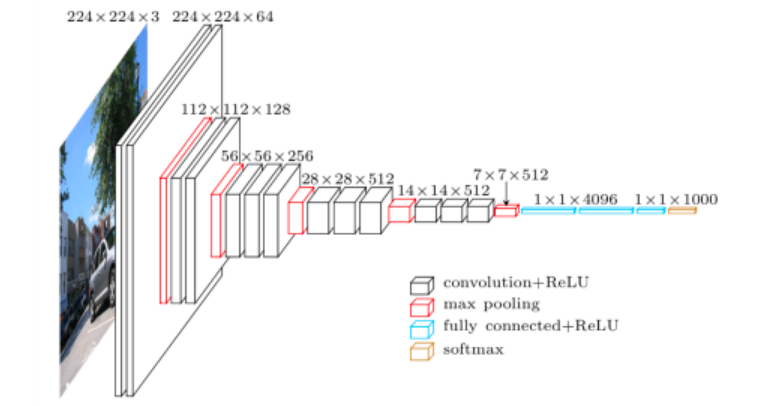
\includegraphics[width = 8.0in]{../images/VGG}}
\centerline{\large Davi Frossard}

\slide{The Fundamental Equation of Deep Learning}

We assume a ``population'' probability distribution $\mathrm{Pop}$ on pairs $(x,y)$.

\vfill
\begin{eqnarray*}
\Phi^* & = & \argmin_\Phi \;E_{(x,y) \sim \mathrm{Pop}}\;{\cal L}(x,y,\Phi) \\
\\
& = & {\color{red} \argmin_\Phi \;E_{(x,y) \sim \mathrm{Pop}}\; -\ln \;P_\Phi(y|x)}
\end{eqnarray*}

\vfill
This loss function ${\cal L}(x,y,\Phi) = - \ln \;P_\Phi(y|x)$ is called {\bf cross entropy loss}.

\slide{Binary Classification}

We have a population distribution over $(x,y)$ with $y \in \{-1,1\}$.

\vfill
We compute a single score $s_\Phi(x)$ where

\vfill
for $s_\Phi(x) \geq 0$ predict $y = 1$

\vfill
for $s_\Phi(x) < 0$ predict $y = -1$

\slide{Softmax for Binary Classification}

\begin{eqnarray*}
  P_\Phi(y|x) & = & \frac{1}{Z} \;e^{ys(x)} \\
  \\
  & = & \frac{e^{ys(x)}}{e^{ys(x)} + e^{-ys(x)}} \\
  \\
  \\
  & = & \frac{1}{1 + e^{-2ys(x)}} \\
  \\
  \\
    & = & {\color{red} \frac{1}{1 + e^{-m(y)}}} \;\;\;\;\;\;m(y|x) = 2ys(x)\;\mbox{is the margin}
\end{eqnarray*}

\slide{Logistic Regression for Binary Classification}

\begin{eqnarray*}
  \Phi^* & = & \argmin_\Phi\;E_{(x,y) \sim \mathrm{Pop}}\;{\cal L}(x,y,\Phi) \\
  \\
  & = & {\color{red} \argmin_\Phi\;E_{(x,y) \sim \mathrm{Pop}}\;-\ln P_\Phi(y|x)} \\
  \\
  & = & \argmin_\Phi\;E_{(x,y) \sim \mathrm{Pop}}\;\ln \left(1 + e^{-m(y|x)}\right) \\
  \\
  \ln \left(1 + e^{-m(y|x)}\right) & \approx & 0 \;\;\;\mbox{for $m(y|x) >> 1$} \\
  \\
  \ln \left(1 + e^{-m(y|x)}\right) & \approx & -m(y|x) \;\;\;\mbox{for $-m(y|x) >> 1$} \\
\end{eqnarray*}

\slide{Log Loss vs. Hinge Loss (SVM loss)}

\centerline{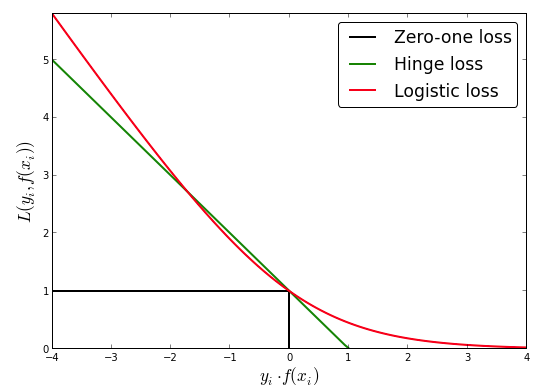
\includegraphics[width = 4.0in]{../images/logloss}}

\slide{Image Classification (Multiclass Classification)}

We have a population distribution over $(x,y)$ with $y \in \{y_1,\;\ldots,\;y_k\}$.

\vfill
$$P_\Phi(y|x) = \softmax_y\;s_\Phi(y|x)$$

\vfill
\begin{eqnarray*}
  \Phi^* & = & \argmin_\Phi\;E_{(x,y) \sim \mathrm{Pop}}\;{\cal L}(x,y,\Phi) \\
  \\
  & = & {\color{red} \argmin_\Phi\;E_{(x,y) \sim \mathrm{Pop}}\;- \ln P_\Phi(y|x)}
\end{eqnarray*}

\slide{Machine Translation (Structured Labeling)}

We have a population of translation pairs $(x,y)$ with $x \in V_x^*$ and $y \in V_y^*$ where
$V_x$ and $V_y$ are source and target vocabularies respectively.

\vfill


\vfill
\begin{eqnarray*}
  P_\Phi(w_{t+1} | x,w_1,\ldots,w_t) & = & \softmax_{w \in V_y \cup \mathrm{<EOS>}} \; s_\Phi(w\;|\;x,w_1,\ldots,w_t) \\
  \\
  \\
  P_\Phi(y|x) & = & \prod_{t = 0}^{|y|} \;P_\Phi(y_{t+1}\;|\;x,y_1,\ldots,y_t)
\end{eqnarray*}

\vfill
\vfill
\begin{eqnarray*}
  \Phi^* & = & \argmin_\Phi \;E_{(x,y) \sim \mathrm{Pop}} \;{\cal L}(x,y,\Phi) \\
  \\
  & = & {\color{red} \argmin_\Phi \;E_{(x,y) \sim \mathrm{Pop}} \;-\ln \;P_\Phi(y|x)}
\end{eqnarray*}

\slide{Entropy, Cross Entropy and KL Divergence}

Let $P$ and $Q$ be two probability distributions on the same set ${\cal Y}$.

\vfill
\centerline{
  $\begin{array}{lrcl}
\mathrm{Entropy}: & H(P) & = & E_{y \sim P}\;-\ln\;P(y) \\
\\
\mathrm{Cross Entropy:} & H(P,Q) & = & E_{y \sim P}\;-\ln\;Q(y) \\
\\
\mathrm{KL\; Divergence:} & KL(P,Q) & = & E_{y \sim P}\;\;\; \ln\;\frac{P(y)}{Q(y)}
  \end{array}$}

\vfill
Cross Entropy Loss:

$${\color{red} E_{(x,y)\sim \mathrm{Pop}}\;-\ln P_\Phi(y|x)}\;\; = \;\; E_{x \sim \mathrm{Pop}}\;H(\mathrm{Pop}(y|x),P_\Phi(y|x))$$

\slide{Jensen's Inequality}

\centerline{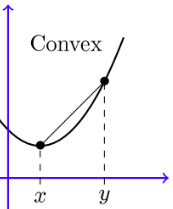
\includegraphics[height = 3.0in]{../images/Jensen}}

\vfill
For $f$ convex (upward curving) we have

\vfill
$$E[f(x)] \geq f(E[x])$$

\slide{KL Divergence}

$$KL(P,Q) \geq 0$$

\vfill
Proof:

\begin{eqnarray*}
  KL(P,Q) & = & \expectsub{y \sim P}{- \log \frac{Q(y)}{P(y)}} \\
  \\
  & \geq & - \log \expectsub{x\sim P}{\frac{Q(y)}{P(y)}} \\
  \\
  & = & - \log \sum_y\; P(y) \frac{Q(y)}{P(y)}  \\
  \\
  & = & - \log \sum_y Q(y) \\
  \\
  & = & 0
\end{eqnarray*}

\slide{Fundamental Equations}

\begin{eqnarray*}
  KL(P,Q) & \geq & 0 \\
  \\
  H(P,Q) & = & H(P) + KL(P,Q) \\
  \\
  \argmin_Q H(P,Q) & = & P
\end{eqnarray*}

\begin{eqnarray*}
  {\color{red} \argmin_{Q(y|x)}\;E_{(x,y)\sim \mathrm{Pop}}\;-\ln Q(y|x)} & = & \argmin_{Q(y|x)}\;E_{x \sim \mathrm{Pop}}\; H(\mathrm{Pop(y|x)}, Q(y|x)) \\
  & = & {\color{red} \mathrm{Pop}(y|x)} \\
\end{eqnarray*}
    
\slide{Asymmetry of Cross Entropy}
Consider 


$$\Phi^* = \argmin_\Phi \;H(P,Q_\Phi)\;\;\;\;\;(1)$$

\vfill
$$\Phi^* = \argmin_\Phi \;H(Q_\Phi,P)\;\;\;\;\;(2)$$

\vfill
For (1) $Q_\Phi$ must cover all of the support of $P$.

\vfill
For (2) $Q_\Phi$ concentrates all mass on the point maximizing $P$.

    
\slide{Asymmetry of KL Divergence}
Consider 


\begin{eqnarray*}
  \Phi^* & = & \argmin_\Phi \;KL(P,Q_\Phi) \\
  & = & \argmin_\Phi\; H(P,Q_\Phi)\;\;\;\;\;\;\;\;\;\;\;\;\;\;\;\;\;\;(1) \\
  \\
  \Phi^* & = & \argmin_\Phi \;KL(Q_\Phi,P) \\
  & = & \argmin_\Phi H(Q_\Phi,P) - H(Q_\Phi)\;\;\;(2)
  \end{eqnarray*}

\vfill
If $Q_\Phi$ is not universally expressive we have that (1) still forces $Q_\Phi$ to cover all of $P$ (or else the KL divergence is infinite)
while (2) allows $Q_\Phi$ to be restricted to a single mode of $P$ (a common outcome).

\slide{END}

}
\end{document}
